% Copyright 2018 Melvin Eloy Irizarry-Gelpí
\setcounter{chapter}{4}
\chapter{Newton's Second Law}
%%%%%%%%%%%%%%%%%%%%%%%%%%%%%%%%%%%%%%%%%%%%%%%%%%%%%%%%%%%%%%%%%%%%%%%%%%%%%%%%
In this experiment you will check the validity of Newton's second law of motion.
%%%%%%%%%%%%%%%%%%%%%%%%%%%%%%%%%%%%%%%%%%%%%%%%%%%%%%%%%%%%%%%%%%%%%%%%%%%%%%%%
\section{Preliminary}
%%%%%%%%%%%%%%%%%%%%%%%%%%%%%%%%%%%%%%%%%%%%%%%%%%%%%%%%%%%%%%%%%%%%%%%%%%%%%%%%
The newtonian approach to describing motion involves concepts like mass, acceleration, and forces. \textbf{Newton's second law} relates these three concepts in a mathematical way:
\begin{itemize}
    \item The amount of \textbf{net force} acting on an object is directly proportional to the amount of \textbf{acceleration} of the object. The constant of proportionality is the \textbf{mass} of the object.
\end{itemize}
In equation form:
\begin{equation}
    F_{\text{net}} = m a
    \label{eq:04.Fma}
\end{equation}
One way to check the validity of Newton's second law would be to measure the net force acting on an object, and also the acceleration resulting from this net force, and check whether the data has a linear shape.
%%%%%%%%%%%%%%%%%%%%%%%%%%%%%%%%%%%%%%%%%%%%%%%%%%%%%%%%%%%%%%%%%%%%%%%%%%%%%%%%
\section{Experiment}
%%%%%%%%%%%%%%%%%%%%%%%%%%%%%%%%%%%%%%%%%%%%%%%%%%%%%%%%%%%%%%%%%%%%%%%%%%%%%%%%
You used an Atwood machine, which is a device involving weights and pulleys. A cart holding a picket fence and a force sensor is attached to a piece of string. The other end of the string has some amount of mass attached to it, that is allowed to hang through a pulley. When the cart is allowed to move, the weight will fall downward and pulled on the string down, and the cart forward. By changing the amount of mass hanging, you can change the amount of net force acting on the cart. You used a photogate to measure the velocity of the cart, and a force sensor to measure the amount of force acting on the cart.
%%%%%%%%%%%%%%%%%%%%%%%%%%%%%%%%%%%%%%%%%%%%%%%%%%%%%%%%%%%%%%%%%%%%%%%%%%%%%%%%
\section{Analysis}
%%%%%%%%%%%%%%%%%%%%%%%%%%%%%%%%%%%%%%%%%%%%%%%%%%%%%%%%%%%%%%%%%%%%%%%%%%%%%%%%
Here are the steps to follow.
%%%%%%%%%%%%%%%%%%%%%%%%%%%%%%%%%%%%%%%%%%%%%%%%%%%%%%%%%%%%%%%%%%%%%%%%%%%%%%%%
\subsection{Calculate the Slope from Velocity and Time}
%%%%%%%%%%%%%%%%%%%%%%%%%%%%%%%%%%%%%%%%%%%%%%%%%%%%%%%%%%%%%%%%%%%%%%%%%%%%%%%%
For each run, the photogate gives you distance, velocity and acceleration data, along with gate state, as they change with time. You are only interested in the velocity and time columns. It is okay that for some time values there is no velocity value listed. This just reflects the fact that the velocity data is not really measured but computed from the time data (along with gate state and knowledge of the size of the picket fence). In any case, a chart with velocity in the vertical axis and time in the horizontal axis looks linear. As done many times before, you can include the best-fit line and find the slope and intercept. The slope corresponds to the \textbf{acceleration} experience by the cart. See the second column in Table \ref{table:04.results} for my results.
%%%%%%%%%%%%%%%%%%%%%%%%%%%%%%%%%%%%%%%%%%%%%%%%%%%%%%%%%%%%%%%%%%%%%%%%%%%%%%%%
\subsection{Calculate the Time-Averaged Force}
%%%%%%%%%%%%%%%%%%%%%%%%%%%%%%%%%%%%%%%%%%%%%%%%%%%%%%%%%%%%%%%%%%%%%%%%%%%%%%%%
For each run, the force sensor gives you the amount of force acting on the cart as time passes. A chart with force in the vertical axis and time in the horizontal axis looks like the amount of force changes over time and thus it is not constant. But a closer look indicates that the values are not changing by a significant amount, and thus this variation is mostly due to random noise. One way to extract a single force value is to calculate the average force over the time period. This is known as the \textbf{time-averaged force}. See the third column in Table \ref{table:04.results} for my results.
%%%%%%%%%%%%%%%%%%%%%%%%%%%%%%%%%%%%%%%%%%%%%%%%%%%%%%%%%%%%%%%%%%%%%%%%%%%%%%%%
\subsection{Calculate the 3-Run Averages}
%%%%%%%%%%%%%%%%%%%%%%%%%%%%%%%%%%%%%%%%%%%%%%%%%%%%%%%%%%%%%%%%%%%%%%%%%%%%%%%%
It is always a good idea to check for consistency by repeating a measurement. With three runs using the same hanging mass, the value of the slope and the time-averaged force should be consistent. You can average each of these three values and obtain your best experimental estimate for the acceleration of the cart, and the amount of force acting on the cart, given an amount of hanging mass. See Table \ref{table:04.averages} for my results.
%%%%%%%%%%%%%%%%%%%%%%%%%%%%%%%%%%%%%%%%%%%%%%%%%%%%%%%%%%%%%%%%%%%%%%%%%%%%%%%%
\subsection{Calculate the Slope from Force and Acceleration}
%%%%%%%%%%%%%%%%%%%%%%%%%%%%%%%%%%%%%%%%%%%%%%%%%%%%%%%%%%%%%%%%%%%%%%%%%%%%%%%%
If you used six different values for the hanging mass, then you should have six pairs of 3-run average acceleration (slope), and 3-run time-averaged force. Make a chart with force in the vertical axis and acceleration in the horizontal axis. Add the best-fit linear function and record the slope value. Based on Equation \ref{eq:04.Fma} the slope should correspond to the total mass of the object moving along the track. This mass is the sum of the mass of
\begin{enumerate}
    \item the picket fence,
    \item the force sensor,
    \item and the cart.
\end{enumerate}
Make sure you use a scale to find these values for your experiment. See Table \ref{table:04.masses} for my case.
%%%%%%%%%%%%%%%%%%%%%%%%%%%%%%%%%%%%%%%%%%%%%%%%%%%%%%%%%%%%%%%%%%%%%%%%%%%%%%%%
\section{My Data}
%%%%%%%%%%%%%%%%%%%%%%%%%%%%%%%%%%%%%%%%%%%%%%%%%%%%%%%%%%%%%%%%%%%%%%%%%%%%%%%%
My data consist of 18 runs:
\begin{itemize}
    \item Runs 1, 2, and 3: 50 g of mass hanging.
    \item Runs 4, 5, and 6: 70 g of mass hanging.
    \item Runs 7, 8, and 9: 80 g of mass hanging.
    \item Runs 10, 11, and 12: 100 g of mass hanging.
    \item Runs 13, 14, and 15: 120 g of mass hanging.
    \item Runs 16, 17, and 18: 150 g of mass hanging.
\end{itemize}
%%%%%%%%%%%%%%%%%%%%%%%%%%%%%%%%%%%%%%%%%%%%%%%%%%%%%%%%%%%%%%%%%%%%%%%%%%%%%%%%
\section{Your Data}
%%%%%%%%%%%%%%%%%%%%%%%%%%%%%%%%%%%%%%%%%%%%%%%%%%%%%%%%%%%%%%%%%%%%%%%%%%%%%%%%
You should have at least three runs for each of at least six different hanging masses.
%%%%%%%%%%%%%%%%%%%%%%%%%%%%%%%%%%%%%%%%%%%%%%%%%%%%%%%%%%%%%%%%%%%%%%%%%%%%%%%%
\newpage
\section{Your Laboratory Report}
%%%%%%%%%%%%%%%%%%%%%%%%%%%%%%%%%%%%%%%%%%%%%%%%%%%%%%%%%%%%%%%%%%%%%%%%%%%%%%%%
Your report should include the following:
\begin{enumerate}
    \item One chart with velocity in the vertical axis, and time in the horizontal axis. Include the best-fit line, and display the equation in the legend.
    \item One chart with force in the vertical axis, and time in the horizontal axis.
    \item A table like Table \ref{table:04.results} with slope and time-averaged force for each run.
    \item A table like Table \ref{table:04.averages} with the 3-run averages.
    \item A table like Table \ref{table:04.masses} with the mass values that you measured.
    \item A chart like Figure \ref{figure:04.fma} with force in the vertical axis and acceleration in the horizontal axis. Include the best-fit line and display the equation for it in the legend.
    \item Calculate the percent difference between the slope from your force versus acceleration chart and the expected total mass value.
    \item Do you find that Newton's second law of motion holds true?
\end{enumerate}
You are free to choose which run to use for items 1 and 2.
%%%%%%%%%%%%%%%%%%%%%%%%%%%%%%%%%%%%%%%%%%%%%%%%%%%%%%%%%%%%%%%%%%%%%%%%%%%%%%%%
\newpage
\section{Tables}
%%%%%%%%%%%%%%%%%%%%%%%%%%%%%%%%%%%%%%%%%%%%%%%%%%%%%%%%%%%%%%%%%%%%%%%%%%%%%%%%
\begin{table}[ht]
    \centering
    \begin{tabular}{|l|r|r|}
        \hline
        \textbf{Run} & \textbf{Slope} (m/s$^{2}$) & \textbf{Time-Averaged Force} (N) \\
        \hline
        1 & 0.67 & 0.426 \\
        2 & 0.66 & 0.426 \\
        3 & 0.62 & 0.431 \\
        \hline
        4 & 0.92 & 0.583 \\
        5 & 0.91 & 0.585 \\
        6 & 0.88 & 0.589 \\
        \hline
        7 & 1.03 & 0.657 \\
        8 & 1.02 & 0.659 \\
        9 & 1.02 & 0.658 \\
        \hline
        10 & 1.27 & 0.800 \\
        11 & 1.25 & 0.797 \\
        12 & 1.26 & 0.796 \\
        \hline
        13 & 1.49 & 0.943 \\
        14 & 1.50 & 0.944 \\
        15 & 1.51 & 0.944 \\
        \hline
        16 & 1.81 & 1.135 \\
        17 & 1.83 & 1.132 \\
        18 & 1.83 & 1.130 \\
        \hline
    \end{tabular}
    \caption{Slope of velocity versus time, and time-averaged force}
    \label{table:04.results}
\end{table}
\vspace{\stretch{1}}
%%%%%%%%%%%%%%%%%%%%%%%%%%%%%%%%%%%%%%%%%%%%%%%%%%%%%%%%%%%%%%%%%%%%%%%%%%%%%%%%
\begin{table}[ht]
    \centering
    \begin{tabular}{|l|r|r|}
        \hline
        \textbf{Runs} & \textbf{Average Slope} (m/s$^{2}$) & \textbf{Average Time-Averaged Force} (N) \\
        \hline
        1, 2, and 3 & 0.65 & 0.427 \\
        4, 5, and 6 & 0.90 & 0.586 \\
        7, 8, and 9 & 1.02 & 0.658 \\
        10, 11, and 12 & 1.26 & 0.798 \\
        13, 14, and 15 & 1.50 & 0.944 \\
        16, 17, and 18 & 1.82 & 1.132 \\
        \hline
    \end{tabular}
    \caption{3-Run Averages}
    \label{table:04.averages}
\end{table}
\vspace{\stretch{1}}
%%%%%%%%%%%%%%%%%%%%%%%%%%%%%%%%%%%%%%%%%%%%%%%%%%%%%%%%%%%%%%%%%%%%%%%%%%%%%%%%
\begin{table}[ht]
    \centering
    \begin{tabular}{|l|r|}
        \hline
        \textbf{Name} & \textbf{Value} (kg) \\
        \hline
        Mass of picket fence & 0.01298 \\
        Mass of force sensor & 0.08775 \\
        Mass of cart & 0.50149 \\
        \hline
        Total mass & 0.60222 \\
        \hline
    \end{tabular}
    \caption{Mass values}
    \label{table:04.masses}
\end{table}
\vspace{\stretch{1}}
%%%%%%%%%%%%%%%%%%%%%%%%%%%%%%%%%%%%%%%%%%%%%%%%%%%%%%%%%%%%%%%%%%%%%%%%%%%%%%%%
\FloatBarrier
\newpage
\section{Figures}
%%%%%%%%%%%%%%%%%%%%%%%%%%%%%%%%%%%%%%%%%%%%%%%%%%%%%%%%%%%%%%%%%%%%%%%%%%%%%%%%
\begin{figure}[ht]
    \centering
    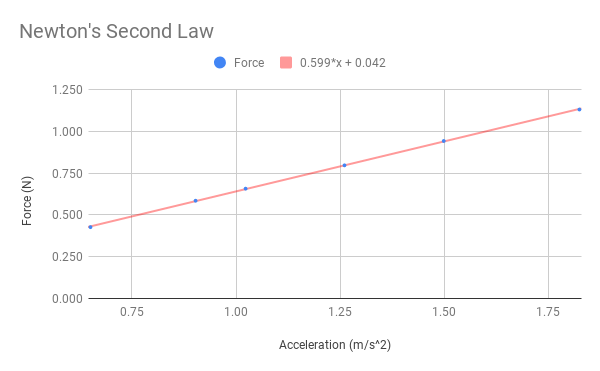
\includegraphics[scale=0.71]{image/04-second-law/newton-2nd-law.png}
    \caption{Force versus Acceleration}
    \label{figure:04.fma}
\end{figure}